% 线性方程的三种情况与统一选解：解的情况与解集、最小二乘、最小范数代表、伪逆、加权与齐次最小二乘、目标的检验条件

\section{线性方程的三种情况与统一选解}
\label{sec:ls-solution-selection}

对同一个方程$\bm A\bm x=\bm b$，本节先用列空间和零空间区分唯一解、无穷多解和无解三种情况，再规定每种情况下要求什么样的解。方程相容时保留全部精确解；不相容时改求离$\bm b$最近的可实现输出，这就是最小二乘；解不唯一时，取欧氏范数最小的一个作代表。三种情况针对原来的精确方程而言，有限维的普通最小二乘问题总有解，其最小范数代表也总是唯一的，所以奇异值分解与伪逆能把各种情形写成同一个公式。随后说明加权与齐次两种变形分别改变了什么目标，最后把各种目标写成可以核对的条件。本节只讨论定义、存在唯一性和最优性，不安排算法过程；怎样把选定的解算出来，从第~\ref{sec:ls-direct-methods}节开始讨论。

\subsection{精确方程的三种情况与解集}
\label{sec:ls-solution-cases}

给定$\bm A\in\mathbb R^{m\times d}$与$\bm b\in\mathbb R^m$，记$\bm a_1,\ldots,\bm a_d$为$\bm A$的各列。由$\bm A\bm x=x_1\bm a_1+\cdots+x_d\bm a_d$，方程$\bm A\bm x=\bm b$问的是能否用$\bm A$的列组合出$\bm b$，以及组合系数是什么。输出$\bm A\bm x$取遍列空间$\operatorname{range}(\bm A)$，所以方程有解当且仅当$\bm b\in\operatorname{range}(\bm A)$，这时称方程\term{相容}（consistent）。把$\bm b$并到$\bm A$右侧得到增广矩阵$[\bm A\;\bm b]$：若$\bm b$已是各列的组合，添上它不扩大列张成的空间，秩不变；否则秩恰好加一。因此
\begin{equation}
 \bm A\bm x=\bm b\ \text{相容}\iff
 \operatorname{rank}[\bm A\;\bm b]=\operatorname{rank}\bm A .
 \label{eq:ls-augmented-rank}
\end{equation}
判据只涉及$\bm b$与列空间的关系，方程个数与未知量个数本身不能决定解的情况。例如两个方程$x=1$、$x=1$多于未知量，却有唯一解；方阵方程$x_1+x_2=1$、$x_1+x_2=2$方程数与未知量数相同，却无解。

方程相容以后，解有几个由零空间决定：两个解之差属于$\ker\bm A$，零空间中的向量加到任何解上也不改变输出。把有没有解和有几个解合起来，得到下面的三分法。

\begin{theorem}[线性方程的三种情况]
\label{thm:ls-three-solution-cases}
设$r=\operatorname{rank}\bm A$，$\tilde r=\operatorname{rank}[\bm A\;\bm b]$。则恰有下面一种情况成立：$\tilde r=r=d$时方程有唯一解；$\tilde r=r<d$时有无穷多解；$\tilde r>r$时无解。
\end{theorem}
\begin{proof}
添上一列至多增加一个方向，所以$\tilde r\in\{r,r+1\}$，三个条件互斥且穷尽。由式~\eqref{eq:ls-augmented-rank}，$\tilde r>r$当且仅当无解。相容时任取一个解$\bm x_0$，全部解为$\bm x_0+\ker\bm A$；由秩零度定理~\ref{thm:ls-rank-nullity}，$\dim\ker\bm A=d-r$，故$r=d$时解唯一，$r<d$时沿任一非零核向量$\bm n$平移得到无穷多个解$\bm x_0+t\bm n$。
\end{proof}

定理中的两种满秩保证不同的事情。$r=d$称为满列秩，它保证至多一个精确解，但不保证有解：$\bm A=(1,1)^\top$满列秩，只有两个分量相等的$\bm b$才相容。$r=m$称为满行秩，此时列空间是整个$\mathbb R^m$，每个右端都有精确解，但解可能不唯一：$\bm A=(1,1)$满行秩，$x_1+x_2=b$的解可沿$(1,-1)^\top$任意平移。方阵满秩时两种保证同时成立，对每个右端恰有一解，这正是$\bm A$可逆的情形。
\phantomsection\label{sec:ls-determinant-invertibility}%
对$d$阶方阵，可逆性也可以由行列式判断：
\[
\begin{gathered}
\bm A\ \text{可逆}\iff\det\bm A\neq0,\\
\bm A^{-1}=\frac{1}{\det\bm A}\operatorname{adj}(\bm A).
\end{gathered}
\]
若$\bm A$可逆，由行列式的乘法性（第~\ref{sec:ls-determinant-properties}节）得$\det\bm A\det(\bm A^{-1})=1$，故$\det\bm A\neq0$；反过来，把古典伴随恒等式$\bm A\operatorname{adj}(\bm A)=\operatorname{adj}(\bm A)\bm A=(\det\bm A)\bm I$（定理~\ref{thm:ls-adjugate-identity}）除以$\det\bm A$，就得到逆矩阵。行列式适合作理论判据；实际计算不展开它，第~\ref{sec:ls-lu}节的消元在求解的同时就能读出秩。

下面用同一个拟合问题依次产生三种情况，本节后面还会回到它。

\begin{example}[直线观测中的三种情况]
\label{ex:ls-line-three-cases}
在$t=0,1,2$处观测一个量，假设它按$a+st$线性变化。未知量$\bm x=(a,s)^\top$，系数矩阵
\[
 \bm A=\begin{bmatrix}1&0\\1&1\\1&2\end{bmatrix}
\]
的第一列对应常数项，第二列对应时刻。取$\bm b=(1,2,3)^\top$，前两个方程给出$a=s=1$，第三个方程也成立；$\bm A$满列秩，所以$(1,1)^\top$是唯一解。把常数列重复为第三列，得到$\widetilde{\bm A}=[\bm a_1\;\bm a_2\;\bm a_1]$，方程成为$(x_1+x_3)+x_2t_i=b_i$；对同一个$\bm b$，三个方程只要求$x_1+x_3=1$、$x_2=1$，秩为$2<3$，有无穷多解。保留原来两列而把观测改为$\bm b=(1,2,2)^\top$，前两个方程仍给出$a=s=1$，第三个方程却要求$3=2$；这时$\det[\bm A\;\bm b]=-1\neq0$，$\tilde r=3>r=2$，三条等式不能同时满足，第~\ref{sec:ls-ordinary-ls}节用最小二乘处理它。
\end{example}

对两种相容情形，给定一个特解$\bm x_p$，由任意两解之差属于$\ker\bm A$，全部解为
\begin{equation}
 \bm x_p+\ker\bm A=\{\bm x_p+\bm n:\bm n\in\ker\bm A\},
 \label{eq:ls-affine-solution-set}
\end{equation}
它是把子空间$\ker\bm A$平移到$\bm x_p$处得到的\term{仿射空间}（affine space），自由度为$d-r$。图~\ref{fig:vol1-add-linear-nullspace-fibers}以$\bm A=(1,1)$画出这种结构。复制常数列的例子中，令$x_3=0$得特解$(1,1,0)^\top$；零空间要求$n_1+n_3=0$、$n_2=0$，由$(1,0,-1)^\top$张成，所以全部解为$\bm x=(1+t,1,-t)^\top$，$t\in\mathbb R$。逐项代回，$\widetilde{\bm A}\bm x$的三个分量是$(1+t)-t=1$、$(1+t)+1-t=2$、$(1+t)+2-t=3$，对每个$t$都等于$\bm b$；唯一的自由参数正对应常数项在两个相同列之间的拆法。核为零时式~\eqref{eq:ls-affine-solution-set}退化为唯一解，核非零时给出仿射解集。这里只建立结构，第~\ref{sec:ls-direct-methods}节的消元与分解把它变成计算过程。

\begin{figure}[!htb]
  \centering
  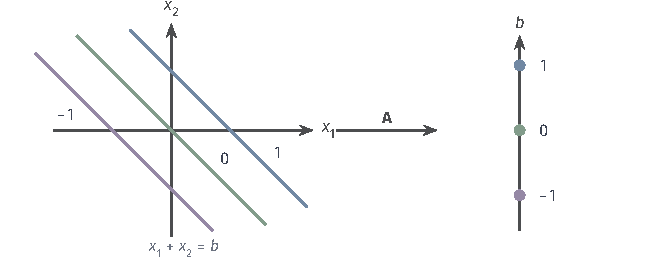
\includegraphics[width=112mm]{figures/00-shared/mathematical-preliminaries-upper/02-linear-spaces/tikz/comprehension-additions/linear-nullspace-fibers.pdf}
  \caption{同一输出对应的整组输入。对$\bm A=(1,1)$，蓝、绿、紫直线分别满足
  $x_1+x_2=1,0,-1$；右侧同色点是各直线的输出。绿色直线是$\ker\bm A$，
  其余直线是它的平移。把一整条直线归为一类后，才得到与可达输出的一一对应。}
  \label{fig:vol1-add-linear-nullspace-fibers}
\end{figure}

\subsection{无精确解时的最小二乘}
\label{sec:ls-ordinary-ls}
\label{sec:ls-least-squares}

当$\bm b$不在列空间中时，没有输入能精确产生它。这时改求使输出误差最小的系数：
\begin{equation}
 \min_{\bm x\in\mathbb R^d}\ \lVert\bm A\bm x-\bm b\rVert_2^2 ,
 \label{eq:linear-algebra-least-squares}
\end{equation}
称为\term{最小二乘}（least squares）问题。问题中有三个对象：系数$\bm x$、拟合值$\bm A\bm x$和残差$\bm r=\bm b-\bm A\bm x$。目标只通过拟合值依赖系数，而拟合值取遍列空间，所以先求列空间中离$\bm b$最近的点，这是\term{子空间最近点}问题。由正交分解（引理~\ref{lem:ls-orthogonal-decomposition}），$\bm b$唯一地写成$\hat{\bm b}+\bm e$，其中$\hat{\bm b}\in\operatorname{range}(\bm A)$，$\bm e\perp\operatorname{range}(\bm A)$。对列空间中任一点$\bm u$，$\hat{\bm b}-\bm u$与$\bm e$正交，勾股关系给出
\begin{equation}
 \lVert\bm b-\bm u\rVert_2^2=\lVert\hat{\bm b}-\bm u\rVert_2^2+\lVert\bm e\rVert_2^2\geq\lVert\bm e\rVert_2^2 ,
 \label{eq:ls-nearest-point-pythagoras}
\end{equation}
等号当且仅当$\bm u=\hat{\bm b}$。所以正交投影$\hat{\bm b}$是唯一的全局最优拟合值，最近点也由“残差与列空间正交”完全刻画。图~\ref{fig:ls-orthogonal-projection-nearest}在一条直线子空间上画出这一几何。

\begin{figure}[htbp]
  \centering
  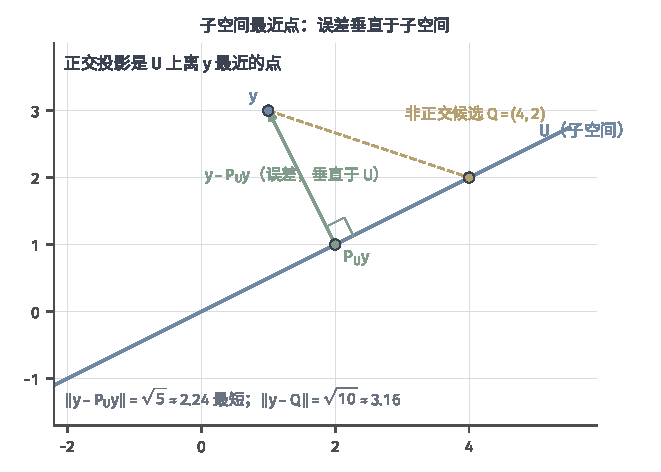
\includegraphics[width=112mm]{figures/00-shared/mathematical-preliminaries-upper/02-linear-spaces/matplotlib/ls-orthogonal-projection-nearest/ls-orthogonal-projection-nearest.pdf}
  \caption{直线子空间$U$（过原点、方向$(2,1)$）上离$\bm y=(1,3)^\top$最近的点是正交投影
  $\bm p=(2,1)^\top$，误差$\bm y-\bm p=(-1,2)^\top$与$U$垂直（直角小方块）；
  同一线上的另一候选$\bm q=(4,2)^\top$到$\bm y$的距离$\sqrt{10}$明显大于最短距离$\sqrt5$。
  这是解析式教学构造。}
  \label{fig:ls-orthogonal-projection-nearest}
\end{figure}

残差与列空间正交，就是与每一列$\bm a_j$正交，合写为$\bm A^\top\bm r=\bm0$。代入$\bm r=\bm b-\bm A\hat{\bm x}$，得到\term{正规方程}（normal equations）
\begin{equation}
 \bm A^\top\bm A\hat{\bm x}=\bm A^\top\bm b .
 \label{eq:linear-algebra-normal-equations}
\end{equation}
“正规”指法向，即残差沿列空间的法方向。由上一段，$\hat{\bm x}$是最小二乘解当且仅当它满足正规方程。这个条件完全由正交分解推出，不需要梯度、Hessian或一般最优化的一阶条件。

拟合值随$\bm b$线性变化，可以写成投影矩阵。设$\bm Q_1$的列是$\operatorname{range}(\bm A)$的一组标准正交基，到列空间的正交投影为$\bm P=\bm Q_1\bm Q_1^\top$（第~\ref{sec:ls-projection-matrices}节），于是拟合值与残差分别是$\bm P\bm b$与$(\bm I-\bm P)\bm b$。$\bm A$满列秩时，由正规方程得$\bm A\hat{\bm x}=\bm A(\bm A^\top\bm A)^{-1}\bm A^\top\bm b$对一切$\bm b$成立，所以
\begin{equation}
 \bm P=\bm A(\bm A^\top\bm A)^{-1}\bm A^\top .
 \label{eq:ls-column-space-projector}
\end{equation}
它对称且幂等：对称说明残差与拟合值正交，幂等说明拟合值再拟合一次不变。这些是几何描述，实际求解只需要系数$\hat{\bm x}$，不必形成这个$m\times m$矩阵。

正规方程是否总有解、有多少个解，仍由列空间与零空间回答。下面的定理把最优性条件、存在性和唯一性合在一起，后面各种最小二乘算法都以它为正确性依据。

\begin{theorem}[最小二乘解的刻画]
\label{thm:ls-least-squares-solutions}
对任意$\bm A\in\mathbb R^{m\times d}$与$\bm b\in\mathbb R^m$，$\hat{\bm x}$是问题~\eqref{eq:linear-algebra-least-squares}的解当且仅当它满足正规方程~\eqref{eq:linear-algebra-normal-equations}。最小二乘解总存在，全部解为$\hat{\bm x}+\ker\bm A$，它们有相同的拟合值$\bm P\bm b$与残差。解唯一当且仅当$\bm A$满列秩，此时$\bm A^\top\bm A$正定，$\hat{\bm x}=(\bm A^\top\bm A)^{-1}\bm A^\top\bm b$。
\end{theorem}
\begin{proof}
由式~\eqref{eq:ls-nearest-point-pythagoras}，$\hat{\bm x}$最优当且仅当$\bm A\hat{\bm x}=\bm P\bm b$。$\bm A\hat{\bm x}$属于列空间，由正交分解的唯一性，这又等价于$\bm b-\bm A\hat{\bm x}\perp\operatorname{range}(\bm A)$，即正规方程。$\bm P\bm b$属于列空间，至少有一个系数向量实现它，所以解存在。若$\bm A^\top\bm A\bm x=\bm0$，则$\lVert\bm A\bm x\rVert_2^2=\bm x^\top\bm A^\top\bm A\bm x=0$，反向包含是直接的，故
\begin{equation}
 \ker(\bm A^\top\bm A)=\ker\bm A ,
 \label{eq:ls-normal-kernel}
\end{equation}
正规方程的解集是一个特解加上$\ker\bm A$，而核向量不改变$\bm A\bm x$。解唯一当且仅当$\ker\bm A=\{\bm0\}$，即满列秩；这时对$\bm x\neq\bm0$有$\bm x^\top\bm A^\top\bm A\bm x=\lVert\bm A\bm x\rVert_2^2>0$，$\bm A^\top\bm A$正定。
\end{proof}

定理区分了两层唯一性：拟合值总是唯一的，系数只在$\bm A$满列秩时唯一。相容方程是残差为零的特例：$\bm P\bm b=\bm b$，最小二乘解集就是精确解集。

\begin{example}[三条不相容观测的最佳折中]
\label{ex:ls-line-least-squares}
回到示例~\ref{ex:ls-line-three-cases}的不相容观测$\bm b=(1,2,2)^\top$。正规方程为
\[
 \begin{bmatrix}3&3\\3&5\end{bmatrix}\hat{\bm x}=\begin{bmatrix}5\\6\end{bmatrix},
\]
解得$\hat{\bm x}=(7/6,1/2)^\top$，残差$\bm r=(-1/6,1/3,-1/6)^\top$。直接核对，$\bm A^\top\bm r$的两个分量为$-\frac16+\frac13-\frac16=0$与$\frac13-\frac26=0$，残差与两列都正交；残差平方和为$1/6$，不为零。三条观测不能同时满足，最小二乘给出它们的最佳折中：中间时刻高于拟合直线，两端低于它。对相容观测$(1,2,3)^\top$，同样的正规方程给出$(1,1)^\top$与零残差，精确求解是最优残差为零的同一目标。
\end{example}

满列秩只保证系数唯一，不保证系数稳定。设计矩阵的两列接近共线时，这一点最明显。

\begin{example}[近共线设计]
\label{ex:ls-nearly-collinear-design}
取非零正交向量$\bm c,\bm q$，设计矩阵的两列为$\bm c$与$\bm c+\varepsilon\bm q$，观测为$\bm y=\bm c+\delta\bm q$。由$w_1\bm c+w_2(\bm c+\varepsilon\bm q)=(w_1+w_2)\bm c+\varepsilon w_2\bm q$，$\varepsilon\neq0$时系数
\[
 \hat{\bm w}=\Bigl(1-\frac{\delta}{\varepsilon},\ \frac{\delta}{\varepsilon}\Bigr)^\top
\]
精确拟合$\bm y$，残差为零；$\varepsilon=0$时两列重合，只能拟合$\bm c$分量，残差跳到$\delta\bm q$，满足$w_1+w_2=1$的系数都是解。
\end{example}

对照三个对象：$\varepsilon\to0$时拟合值从$\bm y$突变为$\bm c$，系数则趋于无穷，并对$\varepsilon$、$\delta$极为敏感。这是近共线几何本身的性质，不是舍入造成的，第~\ref{sec:ls-ls-regularization-sensitivity}节用奇异值量化这种敏感性。

\subsection{多解时的最小范数代表}
\label{sec:ls-select-among-solutions}

最小二乘解集$\hat{\bm x}+\ker\bm A$在秩亏时含无穷多个点，方程本身不指定其中哪一个。为报告一个确定的答案，取欧氏范数最小者。所用的工具是输入空间的正交直和$\mathbb R^d=\operatorname{range}(\bm A^\top)\oplus\ker\bm A$（定理~\ref{thm:ls-four-subspaces-orthogonality}）。

\begin{theorem}[最小范数代表]
\label{thm:ls-minimum-norm-representative}
对任意$\bm A$与$\bm b$，最小二乘解中存在唯一的欧氏范数最小者$\bm x_\star$，它是解集中唯一落在$\operatorname{range}(\bm A^\top)$中的点。方程相容时，$\bm x_\star$是精确解中范数最小者；方程有唯一解时，$\bm x_\star$就是这个解。
\end{theorem}
\begin{proof}
把任一最小二乘解写成$\bm x=\bm x_R+\bm x_N$，$\bm x_R\in\operatorname{range}(\bm A^\top)$，$\bm x_N\in\ker\bm A$。$\bm A\bm x_R=\bm A\bm x$，去掉核分量不改变拟合值，$\bm x_R$仍是最小二乘解。两个解之差属于$\ker\bm A$，它们的行空间分量之差既在$\operatorname{range}(\bm A^\top)$中又在$\ker\bm A$中，只能为零，所以全部解共享同一个$\bm x_\star=\bm x_R$。勾股关系给出$\lVert\bm x\rVert_2^2=\lVert\bm x_\star\rVert_2^2+\lVert\bm x_N\rVert_2^2$，等号当且仅当$\bm x_N=\bm0$。相容与唯一可解的情形是特例。
\end{proof}

选取代表的依据是事先给定的欧氏范数，并没有把多解方程改成唯一可解；换一个范数，选出的点一般也会改变。$\bm A$满行秩时，“落在行空间中”这一刻画可以直接变成公式：所求的解形如$\bm x=\bm A^\top\bm w$，代入方程得$\bm A\bm A^\top\bm w=\bm b$。

\begin{theorem}[满行秩时的最小范数解]
\label{thm:ls-min-norm-full-row-rank}
设$\bm A\in\mathbb R^{m\times d}$满行秩。则$\bm A\bm A^\top$可逆，方程$\bm A\bm x=\bm b$对每个$\bm b$相容，其最小范数解为
\begin{equation}
 \bm x_\star=\bm A^\top(\bm A\bm A^\top)^{-1}\bm b .
 \label{eq:ls-min-norm-full-row-rank}
\end{equation}
\end{theorem}
\begin{proof}
与式~\eqref{eq:ls-normal-kernel}同理，$\ker(\bm A\bm A^\top)=\ker\bm A^\top$，满行秩时它为$\{\bm0\}$，所以$\bm A\bm A^\top$可逆。右端满足$\bm A\bm x_\star=\bm b$，并且落在$\operatorname{range}(\bm A^\top)$中，由定理~\ref{thm:ls-minimum-norm-representative}，它就是最小范数解。
\end{proof}

式~\eqref{eq:ls-min-norm-full-row-rank}说明解是各行的组合，组合系数由$m$阶方程确定。计算时是形成Gram矩阵$\bm A\bm A^\top$，还是对$\bm A^\top$作QR分解，留到第~\ref{sec:ls-normal-equations-method}节与第~\ref{sec:ls-qr-method}节比较。$\bm A$既不满行秩也不满列秩时，两个满秩公式都不能用，下面用奇异值分解写出一般秩下的统一公式。

\subsection{用SVD与伪逆统一选解}
\label{sec:ls-pseudoinverse}

前三小节已经规定了三种方程情形的处理方式：可逆时取唯一解，无解时取最近的拟合值，多解时取范数最小的系数。一般的$\bm A$可能两种选择都要作。本小节沿第~\ref{sec:ls-svd}节的奇异方向给出统一构造：对能够恢复的方向取逆，其他方向保持为零；再用Penrose条件和两个投影核验这一构造的性质。

\subsubsection{伪逆的构造与统一解}
\label{sec:ls-pseudoinverse-construction}

设$\bm A$的秩为$r$，奇异值分解为$\bm A=\sum_{i=1}^r\sigma_i\bm u_i\bm v_i^\top$（式~\eqref{eq:matrix-analysis-svd-rank-one-sum}），$\sigma_1\geq\cdots\geq\sigma_r>0$，并把$\bm u_i$、$\bm v_i$分别扩充为$\mathbb R^m$与$\mathbb R^d$的标准正交基。$\bm A$把$\bm v_i$伸缩为$\sigma_i\bm u_i$，反过来自然应把$\bm u_i$送回$\bm v_i/\sigma_i$。把$\bm b$按$\bm u_i$展开：分量$\bm u_i^\top\bm b$（$i\leq r$）是可以拟合的部分，配给输入方向$\bm v_i/\sigma_i$；$i>r$的分量落在$\operatorname{range}(\bm A)^\perp$中，没有原像，留在残差里；零空间方向$\bm v_{r+1},\ldots,\bm v_d$不分配任何分量。

\begin{definition}[Moore--Penrose伪逆]
\label{def:matrix-analysis-pseudoinverse}
$\bm A$的\term{Moore--Penrose伪逆}（Moore--Penrose pseudoinverse）为
\begin{equation}
 \bm A^\dagger=\sum_{i=1}^r\frac{1}{\sigma_i}\bm v_i\bm u_i^\top ,
 \label{eq:matrix-analysis-pseudoinverse}
\end{equation}
$\bm A=\bm0$时规定$\bm A^\dagger=\bm0$。
\end{definition}

下面的定理说明，这一构造恰好完成了最小二乘与最小范数两次选择。

\begin{theorem}[伪逆给出最小范数最小二乘解]
\label{thm:matrix-analysis-pseudoinverse-minimum-norm}
全部最小二乘解为$\bm A^\dagger\bm b+\ker\bm A$，其中$\bm x_\star=\bm A^\dagger\bm b$是唯一的最小范数解。
\end{theorem}
\begin{proof}
记$b_i=\bm u_i^\top\bm b$、$c_i=\bm v_i^\top\bm x$。由$\bm u_i$标准正交，
\[
 \lVert\bm A\bm x-\bm b\rVert_2^2
 =\sum_{i=1}^r(\sigma_ic_i-b_i)^2+\sum_{i=r+1}^m b_i^2 .
\]
第二项与$\bm x$无关，第一项当且仅当$c_i=b_i/\sigma_i$（$i\leq r$）时为零，$c_{r+1},\ldots,c_d$任取。前者正是$\bm A^\dagger\bm b$的坐标，后者组成任意核向量。$\bm A^\dagger\bm b$只含$\bm v_1,\ldots,\bm v_r$方向，与核向量正交，由定理~\ref{thm:ls-minimum-norm-representative}，它是最小范数解。
\end{proof}

定理对秩和$\bm b$的位置都没有要求，前面的公式都是它的特例。$\bm A$满列秩时核为零，最小二乘解唯一，所以$\bm A^\dagger=(\bm A^\top\bm A)^{-1}\bm A^\top$；满行秩时每个右端都相容，由式~\eqref{eq:ls-min-norm-full-row-rank}，$\bm A^\dagger=\bm A^\top(\bm A\bm A^\top)^{-1}$；$\bm A$可逆时两式都化为$\bm A^{-1}$。一般秩时，两次选择都真正起作用，只有和式~\eqref{eq:matrix-analysis-pseudoinverse}可用。显式写出逆或伪逆只是数学表达，实际计算让分解因子依次作用于右端，步骤见第~\ref{sec:ls-svd-solve}节。

\begin{example}[复制常数列后的最小范数拟合]
\label{ex:ls-line-min-norm}
取示例~\ref{ex:ls-line-three-cases}中的
\[
 \widetilde{\bm A}=\begin{bmatrix}1&0&1\\1&1&1\\1&2&1\end{bmatrix},\qquad \bm b=(1,2,2)^\top .
\]
拟合值$\widetilde{\bm A}\bm x=(x_1+x_3)\bm a_1+x_2\bm a_2$只确定两个常数系数之和。由示例~\ref{ex:ls-line-least-squares}，全部最小二乘解满足$x_1+x_3=7/6$、$x_2=1/2$，即$(7/6-t,\,1/2,\,t)^\top$。范数平方$(7/6-t)^2+t^2+1/4$在$t=7/12$时最小，最小范数代表为$\bm x_\star=(7/12,1/2,7/12)^\top$。它与核方向$(1,0,-1)^\top$的内积为$7/12-7/12=0$，确实落在行空间中。最小二乘选定拟合值，最小范数再在实现它的系数中，把常数项平均分给两个相同的列。
\end{example}

\subsubsection{Penrose条件与两个投影}
\label{sec:ls-penrose-conditions}

奇异向量不唯一，要说明$\bm A^\dagger$与所选分解无关，需要不提奇异向量、又能唯一确定它的条件。

\begin{theorem}[Penrose条件]
\label{thm:ls-penrose-conditions}
$\bm G=\bm A^\dagger$满足
\[
\begin{gathered}
\bm A\bm G\bm A=\bm A,\qquad
\bm G\bm A\bm G=\bm G,\\
(\bm A\bm G)^\top=\bm A\bm G,\qquad
(\bm G\bm A)^\top=\bm G\bm A ,
\end{gathered}
\]
并且满足这四个条件的$\bm G\in\mathbb R^{d\times m}$只有一个。
\end{theorem}
\begin{proof}
由和式与奇异向量的标准正交性，$\bm A\bm A^\dagger=\sum_{i\leq r}\bm u_i\bm u_i^\top$，$\bm A^\dagger\bm A=\sum_{i\leq r}\bm v_i\bm v_i^\top$，二者对称，再右乘$\bm A$或$\bm A^\dagger$即得前两条。反过来设$\bm G$满足四个条件。由第一条，$\bm A\bm G$幂等且$\operatorname{range}(\bm A\bm G)=\operatorname{range}(\bm A)$，再由第三条，它是到$\operatorname{range}(\bm A)$的正交投影；同理$\bm G\bm A$是对称幂等矩阵，零空间为$\ker\bm A$，因而是到$(\ker\bm A)^\perp$的正交投影。正交投影由子空间唯一决定，所以$\bm A\bm G=\bm A\bm A^\dagger$、$\bm G\bm A=\bm A^\dagger\bm A$，于是
\[
 \bm G=\bm G\bm A\bm G=\bm A^\dagger\bm A\bm G=\bm A^\dagger\bm A\bm A^\dagger=\bm A^\dagger .
\]
\end{proof}

四个条件不必死记。前两条是在可恢复方向上的一致性：第一条说明，对能实现的输出$\bm y=\bm A\bm x$，$\bm G\bm y$确实实现它；第二条说明，$\bm G$的输出不含被$\bm A$消去的多余成分。只有前两条时，$\bm A\bm G$与$\bm G\bm A$是幂等矩阵，但可以是斜投影；后两条的对称性要求它们是正交投影，分别对应“取最近的拟合值”和“取范数最小的系数”。正因为四个条件不涉及奇异向量，$\bm A^\dagger$不依赖奇异值分解的选取。

由证明，$\bm A\bm A^\dagger$是到列空间的正交投影，$\bm A^\dagger\bm A$是到行空间$\operatorname{range}(\bm A^\top)$的正交投影。两次选择因此写成两个可以检查的等式：$\bm A\bm x_\star=\bm A\bm A^\dagger\bm b=\bm P\bm b$说明拟合值是$\bm b$在列空间上的投影，$\bm A^\dagger\bm A\bm x_\star=\bm x_\star$说明$\bm x_\star$不含零空间分量。在示例~\ref{ex:ls-line-min-norm}中，$\widetilde{\bm A}\bm x_\star=(7/6,5/3,13/6)^\top$与示例~\ref{ex:ls-line-least-squares}的拟合值相同；$\bm x_\star=\frac7{12}(1,0,1)^\top+\frac12(0,1,0)^\top$已在行空间中，投影不改变它。小正奇异值取倒数后增益$1/\sigma_i$很大，数据误差会被放大，第~\ref{sec:ls-numerical-sensitivity}节再量化这一敏感性；这里先完成各类解的统一表达，为随后选择计算方法提供目标。

\subsection{加权最小二乘}
\label{sec:ls-weighted-ls}

前面都用欧氏长度度量残差，各坐标同等对待。不同观测的可靠程度不同，或观测误差彼此相关时，应按给定的权重度量残差。给定对称正定$\bm M\in\mathbb R^{m\times m}$，\term{加权最小二乘}（weighted least squares）问题为
\begin{equation}
 \min_{\bm x}\ (\bm A\bm x-\bm b)^\top\bm M(\bm A\bm x-\bm b).
 \label{eq:ls-weighted-objective}
\end{equation}
由Gram因子（定理~\ref{thm:ls-gram-factor}）或正定平方根（第~\ref{sec:ls-matrix-square-root}节），可写$\bm M=\bm R^\top\bm R$，$\bm R$可逆，于是目标等于$\lVert\bm R\bm A\bm x-\bm R\bm b\rVert_2^2$。这一步称为\term{白化}（whitening）：先把各坐标的误差变换到同一欧氏尺度，加权问题就成为$\bm R\bm A$、$\bm R\bm b$上的普通最小二乘，定理~\ref{thm:ls-least-squares-solutions}的结论都可以搬过来。

\begin{theorem}[加权最小二乘解的刻画]
\label{thm:ls-weighted-least-squares}
设$\bm M\in\mathbb R^{m\times m}$对称正定。则$\hat{\bm x}$是问题~\eqref{eq:ls-weighted-objective}的解当且仅当它满足加权正规方程
\begin{equation}
 \bm A^\top\bm M(\bm b-\bm A\hat{\bm x})=\bm0 .
 \label{eq:linear-algebra-weighted-normal-equations}
\end{equation}
这组方程总有解，全部解为$\hat{\bm x}+\ker\bm A$；解唯一当且仅当$\bm A$满列秩。
\end{theorem}
\begin{proof}
对$\bm R\bm A$与$\bm R\bm b$应用定理~\ref{thm:ls-least-squares-solutions}：$\hat{\bm x}$最优当且仅当$(\bm R\bm A)^\top(\bm R\bm b-\bm R\bm A\hat{\bm x})=\bm0$，由$\bm R^\top\bm R=\bm M$，这正是式~\eqref{eq:linear-algebra-weighted-normal-equations}。解存在，解集是一个特解加上$\ker(\bm R\bm A)$；$\bm R$可逆，故$\ker(\bm R\bm A)=\ker\bm A$。
\end{proof}

加权正规方程说明残差在$\bm M$内积下与列空间正交。权矩阵改变的是误差的度量，不改变系数和拟合值的含义。若$\bm M$只是半正定，$\ker\bm M$中的残差分量不受惩罚，$\bm R$奇异，唯一性要求$\ker(\bm M\bm A)=\{\bm0\}$，拟合值本身也可能不唯一，正定版本的结论不能全部沿用。

$\bm A$满列秩时，加权拟合值为$\bm P_{\bm M}\bm b$，其中$\bm P_{\bm M}=\bm A(\bm A^\top\bm M\bm A)^{-1}\bm A^\top\bm M$。它幂等，一般不对称，在欧氏内积下是斜投影；但对任意$\bm u,\bm v$，$\bm u^\top\bm M\bm P_{\bm M}\bm v=\bm u^\top\bm M\bm A(\bm A^\top\bm M\bm A)^{-1}\bm A^\top\bm M\bm v$关于$\bm u,\bm v$对称，所以$\bm P_{\bm M}$在$\bm M$内积下自伴，是该内积下的正交投影。同一组$\bm A,\bm b$换用不同权矩阵，最近点随之移动，如下例与图~\ref{fig:linear-algebra-weighted-projection}所示。白化只变换观测端，未知量和它的欧氏范数都不变，所以加权问题与白化后普通问题的解集相同，最小范数代表也一致；构造权因子并调用求解方法的步骤见第~\ref{sec:ls-svd-solve}节。

\begin{example}[同一直线上的两种最近点]
\label{ex:linear-algebra-weighted-projection}
取$\bm A=(1,1)^\top$、$\bm b=(2,1)^\top$，拟合值写成$a(1,1)^\top$。欧氏正规方程$2a=3$给出$(1.5,1.5)^\top$。改用$\bm M=\operatorname{diag}(1,4)$，加权正规方程$5a=6$给出$(1.2,1.2)^\top$：第二个坐标的误差代价更大，最近点向$b_2=1$靠近。加权残差$(0.8,-0.2)^\top$与$(1,1)^\top$的欧氏内积为$0.6$，加权内积为$0.8-4\times0.2=0$，它只在所选内积下正交。
\end{example}

\begin{figure*}[htbp]
  \centering
  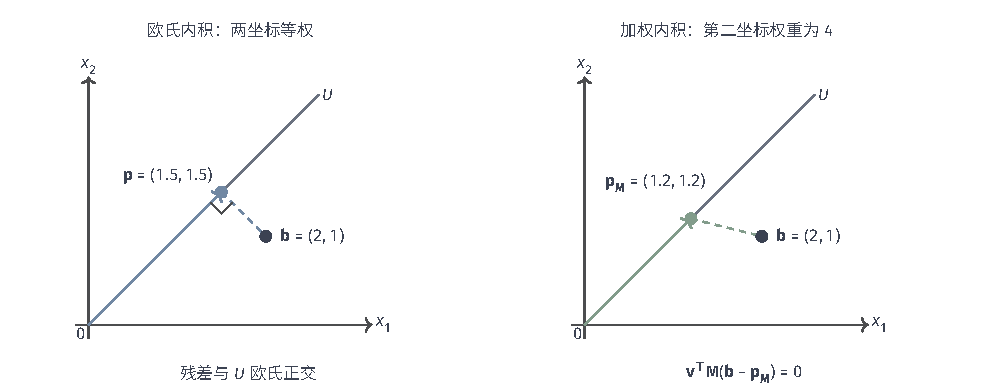
\includegraphics[width=168.998mm]{figures/00-shared/mathematical-preliminaries-upper/02-linear-spaces/tikz/linear-algebra-weighted-projection/figure.pdf}
  \caption{同一目标在同一直线上的欧氏投影与加权投影。实箭头是投影向量，虚线是残差；
  右图画在普通坐标中，残差不必形成欧氏直角。正交性必须用所选内积判断。}
  \label{fig:linear-algebra-weighted-projection}
\end{figure*}

\subsection{齐次最小二乘}
\label{sec:linear-algebra-homogeneous-estimation}

另一类拟合问题的模型写成$\bm A\bm h\approx\bm0$，只确定参数的比例。例如用直线$h_1u+h_2v+h_3=0$拟合平面上的点$(u_j,v_j)$，每个点给出一行$[\,u_j\ v_j\ 1\,]$，$\bm h$乘以非零常数描述同一条直线。直接最小化$\lVert\bm A\bm h\rVert_2^2$总得到无意义的$\bm h=\bm0$，所以必须先固定尺度。固定一个分量，例如$h_3=1$，会把问题化为普通最小二乘，但真实直线过原点时$h_3=0$，这一归一化恰好排除了它。固定欧氏长度则对各分量一视同仁，得到\term{齐次最小二乘}（homogeneous least squares）问题
\begin{equation}
 \min_{\lVert\bm h\rVert_2=1}\ \lVert\bm A\bm h\rVert_2^2
 =\min_{\lVert\bm h\rVert_2=1}\bm h^\top\bm A^\top\bm A\bm h .
 \label{eq:linear-algebra-homogeneous-least-squares}
\end{equation}
它与求齐次方程$\bm A\bm h=\bm0$的全部解不同：后者的解集是子空间$\ker\bm A$，满列秩时只含零向量；前者总给出一个最接近满足的单位方向。

右端是对称半正定矩阵$\bm A^\top\bm A$的Rayleigh商在单位向量上的最小值，正是第~\ref{sec:ls-rayleigh-extremal}节研究的问题。

\begin{theorem}[齐次最小二乘的最优解]
\label{thm:ls-homogeneous-minimizers}
设$\lambda_{\min}$为$\bm A^\top\bm A$的最小特征值。则问题~\eqref{eq:linear-algebra-homogeneous-least-squares}的最小值存在且等于$\lambda_{\min}$，最优解恰为特征空间$\ker(\bm A^\top\bm A-\lambda_{\min}\bm I)$中的单位向量。$\lambda_{\min}$单重时最优解只差一个符号；$\ker\bm A\neq\{\bm0\}$时$\lambda_{\min}=0$，任一单位零空间向量都是最优解。
\end{theorem}
\begin{proof}
由Rayleigh--Ritz定理~\ref{thm:matrix-analysis-rayleigh-ritz}，单位向量上的二次型不小于$\lambda_{\min}$，等号当且仅当该向量属于对应的特征空间。特征空间一维时其中的单位向量只有一对$\pm\bm h_\star$。由式~\eqref{eq:ls-normal-kernel}，$\ker\bm A=\ker(\bm A^\top\bm A)$；它非零时$0$是特征值，而半正定矩阵的特征值非负，故$\lambda_{\min}=0$。
\end{proof}

用$\bm A=[\,1\ -2\,]$核验：$\bm A^\top\bm A$的特征值为$0$与$5$，最小特征值的单位特征向量为$\pm(2,1)^\top/\sqrt5$，它满足$h_1-2h_2=0$，残差为零，两个符号给出同一比例$h_1:h_2=2:1$。

由第~\ref{sec:ls-svd}节，右奇异向量是$\bm A^\top\bm A$的单位特征向量，特征值为奇异值的平方，所以最优解就是最小奇异值对应的右奇异子空间中的单位向量，最小值为最小奇异值的平方。最小特征值接近重根时，任意小的数据扰动都可能从近似最优的子空间中选出不同的方向，最优方向的敏感度由第~\ref{sec:ls-subspace-sensitivity}节的子空间界控制。这里只说明解的性质，用SVD选取具体单位向量的步骤见第~\ref{sec:ls-svd-solve}节。

\subsection{求解目标的检验条件}
\label{sec:ls-least-squares-verification}

算出候选解以后，要用与目标对应的条件核对它。普通最小二乘的最优性条件是$\bm A^\top\bm r=\bm0$，同时报告残差范数$\lVert\bm r\rVert_2$，它是$\bm b$到列空间的距离；要求最小范数解时，再检查$\bm x\perp\ker\bm A$，等价地，$\bm A^\dagger\bm A\bm x=\bm x$。无解方程的最优残差本来就不为零：示例~\ref{ex:ls-line-least-squares}的残差范数为$1/\sqrt6$，它满足$\bm A^\top\bm r=\bm0$，并不说明求解失败。示例~\ref{ex:ls-line-min-norm}中，$(7/6-t,1/2,t)^\top$对每个$t$都满足前两项，只有$t=7/12$满足第三项。

加权问题核对$\bm A^\top\bm M\bm r=\bm0$，报告$\sqrt{\bm r^\top\bm M\bm r}$并说明所用的权矩阵；示例~\ref{ex:linear-algebra-weighted-projection}中欧氏的$\bm A^\top\bm r=0.6\neq0$，这不是错误。齐次拟合不能照搬$\bm A^\top\bm r=\bm0$，否则只会把解推向零向量；应检查$\lVert\bm h\rVert_2=1$，并确认$\bm h$是$\bm A^\top\bm A$最小特征值的特征方向。这些条件规定了后续算法应该达到什么；浮点计算中“为零”要换成相对容限，容限怎样确定、残差小能否保证误差小，在第~\ref{sec:ls-numerical-stability}节讨论，直接法的分解质量与迭代法的停止条件分别见第~\ref{sec:ls-direct-method-comparison}节、第~\ref{sec:ls-stationary-stopping}节和第~\ref{sec:ls-krylov-stopping}节。
